\chapter{Methods}
\label{chapter:methods}
% \thispagestyle{fancy}

\section{Reconstruction of a neuronal network}
\label{reconstruction}
First of all, we chose to reconstruct the neuronal network based on a single neuron, a fast-spiking interneuron. \href{https://neuromorpho.org/}{NeuroMorpho.Org} \cite{Neuromorpho1,Neuromorpho2} is an archive containing multiple reconstructions of different types of neurons from across different researches. The choice was completely arbitrary and was made to simplify the biological complexity of the problem while keeping the computational complexity because fast-spiking interneurons allow the creation of any kind of synapse. The exact neuron was "NMO\_36576" from one research of 2013 \cite{interneuron}, the figure \ref{fig:interneuron} contains a representation of this neuron. This specimen belonged to the subiculum of a rat and one characteristic of note is that the neuron spatial distribution is not uniformed, $298.75 \mu m$ x $538.69 \mu m$ x $66.28 \mu m$.
\begin{figure}[h!]
    \centering
    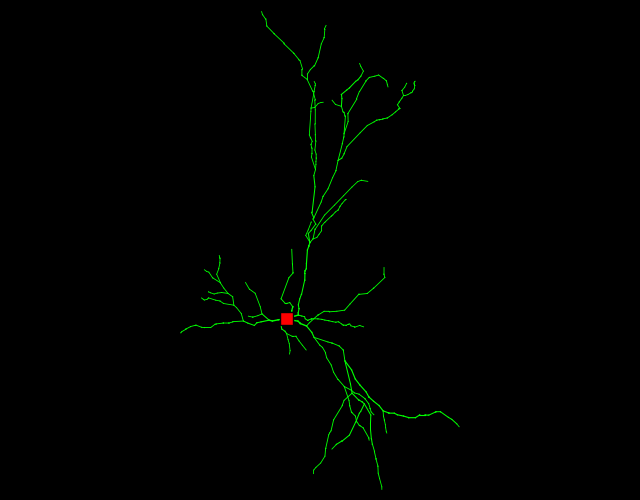
\includegraphics[width=0.75\textwidth]{figures/interneuron.png}
    \caption{Fast-spiking interneuron used in the thesis.}
    \label{fig:interneuron}
\end{figure}

To avoid reading the SWC file every time that it was needed to replicate the neuron, it was designed another file called RPL. This new format file defined a neuron per line and each line contained which transformations were going to be applied. The possible transformations defined were rotation and translation. Scaling and shearing were discarded because they deform the morphological definition of the neuron. A transformation was defined by three values: the first value defined which transformation (0 for translation and 1 for rotation), the second value defined which axis (0 means axis x, 1 means axis y, 2 means axis 3) and the third value defined the amount of transformation in micrometres for translation and radians for rotation. Any amount of transformation could be concatenated, so every possible neuron was possible.

\section{Data structure and construction algorithm}
\subsection{$k$-d tree}
When building a $k$-d tree are necessary a list of the points and a depth. As shown in algorithm \ref{alg:buildtree}, if the list of nodes is empty, we have finished building the tree and it is none. Otherwise, it first needs to find the dimension along which the splitting plane (or hyperplane) is going to be defined and then it chooses a point to create the plane (or hyperplane). Then, the algorithm divides the space into two subsets that are at the left or the right of the plane (or hyperplane) along that dimension. Finally, it creates the subtrees recursively increasing the depth by one. The returned node needs to contain not only the point and the left and right subtree but also the splitting dimension, so when performing a spatial-query, it is possible to know which dimension is responsible for the branches. 
\begin{algorithm}[h!]
    \caption{Constructs a $k$-d tree
        \label{alg:buildtree}}
    \begin{algorithmic}[1]
    \Require{$N$ is the list of points to construct the $k$-d tree with.}
    \Require{$k$ is the depth of the $k$-d tree.}
    \Statex
    \Function{BuildTree}{$N, k$}
        \If{$|N| = 0$}
            \State \Return{nullptr}
        \EndIf
        \State $d$, $p$ $\gets$ SplittingFunction($N, k$) \Comment{$d$ is the splitting dimension and $p$ is the point}
        \State LeftSplit  $\gets \{ n \in N\, |\, n_d \leq p_d \land n \neq p \} $ 
        \State RightSplit $\gets \{ p \in N\, |\, p_d   <  n_d \land n \neq p \} $ 
        \State LeftChild  $\gets$ \Call{BuildTree}{$LeftSplit, k+1$}
        \State RightChild $\gets$ \Call{BuildTree}{$RightSplit, k+1$}
        \State \Return{new \Call{Node}{$p$,$d$,LeftChild,RightChild}}
    \EndFunction
    \end{algorithmic}
\end{algorithm}

\pagebreak

\section{Splitting function and heuristics}
The canonical and original method for dividing the list of nodes is really simple and still leaves a lot of room for improvement. That is the reason because there are several studies trying to improve the splitting function for different applications. This thesis studied how the proposed splitting functions work for the touching point detection.

\subsection{Canonical splitting function}
The canonical method was first described whit the $k$-d tree in its original paper \cite{Bentley}. This method selects the splitting dimension by round-robin, that means the dimension cycles along all the axis. For example, in a 3D tree, the first plane will be aligned with the x-axis, the root's children will both have y-aligned planes, the grandchildren's planes will be aligned with the z-axis, the root's great-grandchildren will all have x-aligned planes, and so on. Once the axis is chosen, the algorithm chooses the median point in that axis from all the points. One possible implementation of this algorithm is the algorithm \ref{alg:canonical}.
\begin{algorithm}[h!]
    \caption{Canonical splitting function
        \label{alg:canonical}}
    \begin{algorithmic}[1]
    \Require{$N$ is the list of points to construct the $k$-d tree with.}
    \Require{$k$ is the depth of the $k$-d tree.}
    \Require{$K$ is the number of dimensions.}
    \Statex
    \Function{SplittingFunction}{$N, k$}
        \State axis $\gets \pmod{K}$ 
        \State \textbf{select} median \textbf{by} axis \textbf{from} N
        \State \Return{(axis,median)}
    \EndFunction
    \end{algorithmic}
\end{algorithm}

The main advantage of this method is that it leads to a balanced $k$-d tree, that means that each leaf of the tree is approximately at the same distance to the root. Selecting the median is a complex task were different approaches can be done. Sorting all the points with a sorting algorithm such as heapsort or mergesort, will lead into a complexity $\mathcal{O}(n\log{}n)$. An improved solution with complexity $\mathcal{O}(n)$ called PICK \cite{BLUM1973448} can be also implemented. A common implementation that is approximate selects random points from the total of points and use the median of those points. Although it is not optimal and does not ensure a balanced tree, it is widely used and often results in nicely balanced trees. In this thesis, we have used a built-in function from C++11 called "std::nth\_element". It is a partial sorting algorithm that rearranges the elements in the vector such as the element pointed at by the $n^{th}$ is changed so it would occur in that position if the vector was sorted, all elements before are less than or equal to the new $n^{th}$ element and the complexity is linear to the number of elements $\mathcal{O}(n)$ \cite{C++11iso}.

\subsection{Surface area heuristic}
The surface area heuristic (SAH) was proposed by MacDonald and Booth in their paper of 1990 \cite{MacDonald1990-jo}. The main idea behind their proposal is that the number of rays likely to intersect a convex object is roughly proportional to its surface area, assuming that the ray origins and directions are uniformly distributed throughout the space. We believed there was a similarity with our task because our neurons are uniformly distributed in the space, and the orientation of the touching point does not matter, so it can be said that the "ray direction" is also evenly distributed. Instead of using the straight-forward implementation from the original description of the algorithm that is $\mathcal{O}(n^2)$ for building the tree, we have used other implementation \cite{WaldHavran06} that is $\mathcal{O}(n \log^2{}n)$. This implementation is the algorithm \ref{alg:sah}.
\begin{algorithm}[h!]
    \caption{Surface area heuristic
        \label{alg:sah}}
    \begin{algorithmic}[1]
    \Require{$N$ is the list of points to construct the $k$-d tree with.}
    \Require{$k$ is the depth of the $k$-d tree.}
    \Require{$K$ is the number of dimensions.}
    \Statex
    \Function{SplittingFunction}{$N, k$}
        \State $\^{C}, \^{d}, \^{p} \gets (\infty, \infty, \emptyset)$
        \For{$i = 1..K$}
            \State $E \gets \emptyset$
            \ForAll{$p \in N$}
                \State $E \gets E \cup (p,p_i,+) \cup (p,p_i,-)$ \label{alg:sah:change}
            \EndFor
            \State \Call{sort}{$E$} \Comment{First, it orders by $p_i$ and if they are equal, then it goes first the $-$ and then the $+$}
            \State $N_l, N_p, N_r \gets (0,0,|N|)$
            \For{$j = 1..|E|$}
                \State $p \gets E_{j,p}$
                \State $p^{+},p^{-},p^{|} \gets 0$
                \While{$j < |E| \land E_{j,\xi} = p_\xi \land E_{j,type} = - $}
                    \State $p^{-} \gets p^{-} + 1$
                    \State $j \gets j + 1$
                \EndWhile
                \While{$j < |E| \land E_{j,\xi} = p_\xi \land E_{j,type} = |$}
                    \State $p^{|} \gets p^{|} + 1$
                    \State $j \gets j + 1$
                \EndWhile
                \While{$j < |E| \land E_{j,\xi} = p_\xi \land E_{j,type} = + $}
                    \State $p^{+} \gets p^{+} + 1$
                    \State $j \gets j + 1$
                \EndWhile
                \State $N_p \gets p^{|}$
                \State $N_r \gets N_r - p^{|} - p^{-}$
                \State $C \gets SAH(p,N_l,N_r,N_p)$ \label{alg:sah:sah}
                \If{$C < \^{C}$}
                    \State $\^{C}, \^{d}, \^{p} \gets (C, i, p)$
                \EndIf
                \State $N_l \gets N_l + p^{+} + p^{|}$
                \State $N_p \gets 0$
            \EndFor
        \EndFor
        \State \Return{$(\^{d},\, \^{p})$}
    \EndFunction
    \end{algorithmic}
\end{algorithm}

 The called function in line \ref{alg:sah:sah}, SAH, basically is defined as:
\begin{align*}
  SAH(p,N,N_l,N_r,N_p) = \lambda * (K_T + min(&\frac{(N_l+N_p)|\{t\in N\, |\, t_i < p_i\}|+N_r|\{t\in N\, |\, t_i > p_i\}|}{|N|},\\
  &\frac{N_l|\{t\in N\, |\, t_i < p_i\}|+(N_p+N_r)|\{t\in N\, |\, t_i > p_i\}|}{|N|}))
\end{align*}
There are two values in this function that are unknown $\lambda$ and $K_T$, $\lambda$ is a factor to prioritize cutting empty space, and it will be $0.8$ if $N_l$ or $N_r$ is $0$, otherwise it is $1$. $K_T$ is a constant that represents the cost of a transversal step in the tree. We stablished it to $0.2$ based on other paper \cite{Yucheng}. The implemented version is not exactly the proposed in the original article. In line \ref{alg:sah:change}, they firstly clamp the triangle containing the point and in case the resulting triangle is planar, then it changes what is added to $E$, by $E \cup (p, p'_{min,k}, |)$. We have done this because we are creating one $k$-d tree per neuron, so the neuron will always be inside the voxel of the $k$-d tree.


\subsection{Curve complexity heuristic}
The curve complexity heuristic propose a new splitting function based on SAH to optimize $k$-d trees for curves abstractions \cite{Yucheng}. The main idea behind their proposal is to adapt SAH so they can perform radius nearest curve search better. We believed there is a great similarity between their proposal and our problem because we also want to find all the nearest neurons given a query point $\mathbf{q}$ and a distance $\mathbf{r}$. A possible implementation could be the algorithm \ref{alg:cch}.
\begin{algorithm}[h!]
    \caption{Curve complexity heuristic
        \label{alg:cch}}
    \begin{algorithmic}[1]
    \Require{$N$ is the list of points to construct the $k$-d tree with.}
    \Require{$k$ is the depth of the $k$-d tree.}
    \Require{$K$ is the number of dimensions.}
    \Statex
    \Function{SplittingFunction}{$N, k$}
        \State $\^{C} \gets \infty$
        \State $\^{p} \gets \emptyset$
        \State $\^{d} \gets \emptyset$
        \For{i = 1..K}
            \State $C_i \gets 0$ \Comment{$C(T) = C_{\text{traversal}}(T)+C_{\text{backtrack}}(T)-nT_{\text{dist}}$}
            \State \textbf{select} median \textbf{by} axis \textbf{from} N
            \Statex
            \Comment{$C_{\text{trasversal}}(T) = T_{\text{trasversal}} + [P(T_l|T)l+P(T_r|T)r]T_{\text{dist}}$}
            \State $C_i \gets 0.2 + l*\frac{\text{Volume}(\{p \in N\, |\, p_i < \text{median}_i\})}{\text{Volume}(N)} + r*\frac{\text{Volume}(\{p \in N\, |\, p_i > \text{median}_i\})}{\text{Volume}(N)}$  
            
            \Comment{$C_{\text{backtracl}}(T) = \lambda(\log{\frac{1}{\rho}(n)+\log{\frac{1}{\tau}}(n)})/2$}
            \Comment{$\rho := \frac{l}{n}$, $\tau := \frac{r}{n}$}
            \State $C_i \gets C_i + \lambda*(\frac{\log{}(n)}{\log{}(\frac{|\{p \in N\, |\, p_i < \text{median}_i\}|}{|N|})} + \frac{\log{}(n)}{\log{}(\frac{|\{p \in N\, |\, p_i > \text{median}_i\}|}{|N|})})$
            \If{$C_i < \^{C}$}
                \State $\^{C} \gets C_i$
                \State $\^{p} \gets \text{median}$
                \State $\^{d} \gets i$
            \EndIf
        \EndFor
        \State \Return{$(\^{d},\, \^{p})$}
    \EndFunction
    \end{algorithmic}
\end{algorithm}

In their paper, they do not study the time complexity of their solution, so we are going to do it. Assuming that the volume functions and selecting the median are $\mathcal{O}(n)$ and the other operations are $\mathcal{O}(1)$. To obtain the cost function, it will sum the cost of finding the median ($n$), the find of the volumes function ($n$), the cost of splitting ($2n$) and the cost of constructing the subtrees recursively ($2T(\frac{n}{2})$):
\begin{align*}
    T(n) &= n + n + 2n + 2T(\frac{n}{2})\\
    &= 4n + 2T(\frac{n}{2}) \\
    &= 4n + 2[4\frac{n}{2} + 2T(\frac{n}{4})] = 8n + 4T(\frac{n}{4}) \\
    &= 8n + 4[4\frac{n}{4} + 2T(\frac{n}{8})] = 12n + 8T(\frac{n}{8}) \\
    &= 12n + 8[4\frac{n}{8} + 2T[\frac{n}{16}]] = 16n + 16T(\frac{n}{8}) \\
    &= \dots = 4*i*n + 2^iT(\frac{n}{2^i}), i \in \mathbb{Z}^+ \\
    &\text{This ends when $\frac{n}{2^i} = 1$, because $T(1)\in\mathcal{O}(1)$} \\
    &n = 2^i \implies i = \log{}(n) \\
    &\text{Therefore, if we substitute in the last one, we get} \\
    T(n) &= 4n\log{}(n)+2^{\log{}(n)} = 4n\log{}(n)+n \in \mathcal{O}(n\log{}(n))
\end{align*}

\subsection{Median of the hyperplane with maximum variance}
This heuristic is our own proposal and is similar to curve complexity heuristic, because it chooses the splitting point by the median and our heuristic defines the splitting dimension. The main idea behind our proposal is that the dimension with a higher variance means that the points are more separated between them and therefore if we split, we are improving. To avoid a costly implementation of the variance, we have implemented the algorithm proposed by Donald Knuth in his book "The art of computer programming. Vol. 2" \cite{knuth97} (page 232). So, the algorithm implemented can be seen in the algorithm \ref{alg:maxvariance}.
\begin{algorithm}[h!]
    \caption{Median of the hyperplane with maximum variance
        \label{alg:maxvariance}}
    \begin{algorithmic}[1]
    \Require{$N$ is the list of points to construct the $k$-d tree with.}
    \Require{$k$ is the depth of the $k$-d tree.}
    \Require{$K$ is the number of dimensions.}
    \Statex
    \Function{SplittingFunction}{$N, k$}
        \State $n \gets 0$
        \State $M \gets \{0,0,0\}$
        \State $S \gets \{0,0,0\}$
        \ForAll{$p \in N$}
            \State $n \gets n + 1$
            \For{i = 1..K}
                \State $\delta \gets p_i - M_i$
                \State $M_i \gets M_i + \frac{\delta}{n}$
                \State $S_i \gets S_i + \delta*(p_i - M_i)$
            \EndFor
        \EndFor
        \State $d \gets $ \Call{max\_element}{$S$} \Comment{max\_element returns the index of the max element in S}
        \State \textbf{select} median \textbf{by} $d$ \textbf{from} $N$
        \State \Return{(d,p)}
    \EndFunction
    \end{algorithmic}
\end{algorithm}

The time complexity of this function is trivially $\mathcal{O}(n)$, and therefore when added to the building tree function it is also $\mathcal{O}(n\log{}(n))$ as the other heuristics.
\pagebreak

\subsection{Minimum variance union}
This heuristic is also our own proposal and it is an improvement from the previous. It also uses the variance of the points in that dimension as a guide, but in this case it tries to minimize the void. To do so, it will minimize for all the points the sum of the variances at the left subset and the right subset. To avoid go through all the points twice, it calculates all the variance at the same time using memoization. The porposed algorithm works as follow \ref{alg:minvariance}.
\begin{algorithm}[h!]
    \caption{Minimum variance union
        \label{alg:minvariance}}
    \begin{algorithmic}[1]
    \Require{$N$ is the list of points to construct the $k$-d tree with.}
    \Require{$k$ is the depth of the $k$-d tree.}
    \Require{$K$ is the number of dimensions.}
    \Statex
    \Function{SplittingFunction}{$N, k$}
        \State $\^{S} \gets \infty$
        \State $\^{p} \gets \emptyset$
        \State $\^{d} \gets \emptyset$
        \For{i = 1..K}
            \State \Call{sort_by_dimension}{N,i}
            \State $S_l \gets $ Array of size $|N|$ with $0$
            \State $S_r \gets $ Array of size $|N|$ with $0$
            \State $M_l \gets $ Array of size $|N|$ with $0$
            \State $M_r \gets $ Array of size $|N|$ with $0$
            \Statex
            \For{$j \in [1,|N|)$}
                \State $\delta \gets N_{j,i} - M_{l,j-1}$
                \State $M_{l,j} \gets \delta / (i+1)$
                \State $S_{l,j} \gets \delta *  N_{j,i} - M_{l,j}$ \Comment{Compute the variance left to right}
                \Statex
                \State $\delta \gets N_{|N|-j-1,i} - M_{l,|N|-j}$
                \State $M_{r,|N|-j-1} \gets \delta / (i+1)$
                \State $S_{r,j} \gets \delta *  N_{|N|-j-1,i} - M_{r,|N|-j-1}$ \Comment{Compute the variance right to left}
            \EndFor
            \For{$j \in [0,|N|)$}
                \If{$S_{l,j} + S_{r,j} < \^{S}$}
                    \State $\^{S} \gets S_{l,j} + S_{r,j}$
                    \State $\^{p} \gets N_j$
                    \State $\^{d} \gets i$
                \EndIf
            \EndFor
        \EndFor
        \State \Return{$(\^{d},\, \^{p})$}
    \EndFunction
    \end{algorithmic}
\end{algorithm}

The time complexity of this function is trivially $\mathcal{O}(n)$, and therefore when added to the building tree function it is also $\mathcal{O}(n\log{}(n))$ as the other heuristics.
\pagebreak

\section{Neuron touch point task}
Due to the fact that the implemented solution uses one $k$-d tree per neuron, the neuron touch point task is trivial to implement, because it only needs to look for if there is a point which distance to the query point is less than a certain threshold. In our case, we choose that threshold to be $3 \mu m$, but it is a variable of our search function (algorithm \ref{alg:find}).
\begin{algorithm}[h!]
    \caption{Touchpoint query
        \label{alg:find}}
    \begin{algorithmic}[1]
    \Require{$\text{root}$ is a $k$-d tree, $\text{root}_p$ is the point represented in the node, $\text{root}_d$ is the splitting dimension, $\text{root}_l,\, \text{root}_r$ are the left and right children.}
    \Require{$q$ is the query point where the touching point is looked for.}
    \Require{$\text{dist}$ is the distance to define a touching point.}
    \Statex
    \Function{FindTouchpoint}{$\text{root},\, q,\, \text{dist}$}
        \If{root $=$ nullptr}
            \State \Return{nullptr}
        \EndIf
        \State $\delta \gets |\text{root}_p - q|$
        \If{$\delta \leq$ dist}
            \State \Return{root}
        \Else
            \If{$q_{\text{root}_d} \leq \text{root}_{\text{root}_d}$}
                \State res $\gets$ FindTouchpoint($\text{root}_l,\, q,\, \text{dist}$)
                \If{res $\ne$ nullptr}
                    \State \Return{res}
                \EndIf
                \If{$ \text{root}_{\text{root}_d} - q_{\text{root}_d} \leq \text{dist}$}
                    \State res $\gets$ FindTouchpoint($\text{root}_r,\, q,\, \text{dist}$)
                    \If{res $\ne$ nullptr}
                        \State \Return{res}
                    \EndIf
                \EndIf
            \Else
                \State res $\gets$ FindTouchpoint($\text{root}_r,\, q,\, \text{dist}$)
                \If{res $\ne$ nullptr}
                    \State \Return{res}
                \EndIf
                \If{$q_{\text{root}_d} - \text{root}_{\text{root}_d} \leq \text{dist}$}
                    \State res $\gets$ FindTouchpoint($\text{root}_l,\, q,\, \text{dist}$)
                    \If{res $\ne$ nullptr}
                        \State \Return{res}
                    \EndIf
                \EndIf
            \EndIf
            \State \Return{nullptr}
        \EndIf
    \EndFunction
    \end{algorithmic}
\end{algorithm}


On a sight, it is trivial to see that the computational cost in the worst case is $\mathcal{O}(n)$, but that probably in average will be $\mathcal{O}(\log{}(n))$ because every time that the algorithm branches, it can discard the half of the data points.
\pagebreak

\section{Task parallelization}
\href{https://www.openmp.org/}{OpenMP} 5.2 was used to introduce parallel programming. OpenMP is an API to implement shared-memory multiprocessing programming in C, C++ and Fortran. To avoid any race condition and to maximize the parallelization of the processes, it was only applied when there were no shared resources between the possible sub-processes. It was widely used for creating the subtrees, where every time that it was needed to call recursively the building function with a subset of the data points, it was done with parallel tasks. Also, when performing the query makes use of parallelizing the search of all the k-d trees.

\section{Test cases
    \label{methods:tests}}
Firstly, the distance to define a touchpoint was fixed to $3 \mu m$. Although it could seem to be arbitrary, it was the middle value between $0.5 \mu m$ and $5 \mu m$, the range proposed by other studies \cite{10.3389/fncom.2015.00120, doi:10.1073/pnas.1202128109}. Once the distance to define a touchpoint was fixed, there were two possible variables to vary for benchmarking the scalability of the data structure and heuristics. The variable for each test case is the number of neurons of the neuronal network given the density and the neuron density of the search space given the number of neurons.

In order to reach realistic values for the number of neurons, we fixed the density to 16991 neurons/$mm^3$ \cite{Trujillo-Estrada2014-uv}, but there could be other densities such us 2048neurons/$mm^3$ and 2790neurons/$mm^3$ \cite{Keller2018-dm} according to our neuron that is a fast-spiking interneuron in the subiculum. The number of neurons was a range between 150 neurons and 85000 neurons. This number is lower than the total amount of any type of neurons in the subiculum of a rat brain which is between 46000 and 330000 neurons \cite{Mulders1997-bh}.

For the other test case, the number of neurons was fixed to 25230 neurons, so it does not have a high time cost. Then the density of neurons by $mm^3$ was defined in a range of 50 neurons/$mm^3$ and 20000 neurons/$mm^3$. The value of the upper bound was chosen to keep realistic densities \cite{Keller2018-dm}. Another test case was derivated with higher densities, between 50000 neurons/$mm^3$ and 500000 neurons/$mm^3$, to be able to extrapolate the results to other types of neurons and regions of the brain.

For the purpose of creating the tests of every test case, we developed a script (algorithm \ref{alg:rpl_files}) that given a density and the number of neurons, it will rotate randomly each neuron and then translate it into the space so the distance of the origin of all the neurons is in a grid such as the distance between them maintains the density. This system uses the RPL files explain in section \ref{reconstruction}.

\begin{algorithm}[h!]
    \caption{Create a test
        \label{alg:rpl_files}}
    \begin{algorithmic}[1]
    \Require{$N$ is the number of neurons to use in the test}
    \Require{$D$ is the density in neurons/$mm^3$ to use in the test}
    \Procedure{CreateTest}{$N, D$}
        \State $\delta \gets 1000*\sqrt[3]{\frac{1}{D}}$
        \State $n_1 \gets \lfloor \sqrt[3]{N} \rceil$
        \State $n_2 \gets \lfloor \sqrt{\frac{N}{n_1}} \rceil$
        \State $n_3 \gets \lfloor \frac{N}{n_1n_2} \rceil$
        \For{i = 1..$n_1$}
            \For{j = 1..$n_2$}
                \For{k = 1..$n_3$}
                    \State rotation $\gets$ \Call{RndChoice}{[[], [0], [1], [2], [0,1], [0,2], [1,2], [0,1,2]]}
                    \State rotation $\gets$ \Call{RndShuffle}{rotation}
                    \ForAll{$r \in \text{rotation}$}
                        \State $\phi \gets$ \Call{RndUniform}{$-\pi,\, \pi$}
                        \State \Call{Write}{'\{\} \{\} \{\}\,'.format(1, $r$, $\phi$)}
                    \EndFor
                    \State \Call{Write}{'0 0 \{\} 0 1 \{\} 0 2 \{\}\textbackslash n'.format($\delta*i$, $\delta*j$, $\delta*k$)}
                \EndFor
            \EndFor
        \EndFor
    \EndProcedure
    \end{algorithmic}
\end{algorithm}


\section{Computer specification}
During this project, we used a personal computer running Debian Live 11.3.0 Standard with an architecture Amd64. The processor is an AMD FX(tm)-8350 with eight cores, 8 threads, working at 4.0 GHz, 384KB of caché L1, 8MB of caché L2 and 8MB of caché L3. Furthermore, it has 16 GB of DDR3 RAM at 1600 MHz distributed in 3 modules: one module of 8 GB (Kingston KHX1600C9D3K2/8GX) and two modules of 4 GB (Kingston 99U5584-012.A00LF). We hadn't physical access to the computer, so it runs an OpenSSH server.